\ifx\ucebnice\undefined
\documentclass[a5paper,10pt,twoside]{book}
\usepackage{luatex85}
\usepackage{latexsym}
\usepackage{amsmath}
\usepackage{amsfonts}
\usepackage{amsthm}
\usepackage{amssymb}
\usepackage{fncylab}
\usepackage{comment}
\usepackage{float}
\usepackage{wrapfig}
\usepackage{tikz}
\usepackage{tikz-qtree}
\usepackage{url}
\usepackage{xcolor}
\usepackage{pdfpages}
\usepackage[czech]{babel}
\definecolor{svlinks}{rgb}{.0,0.3,0.6} %tmavě modrá
\usepackage[bookmarks, colorlinks=false,pdfhighlight=/O,linkcolor=svlinks,urlcolor=svlinks,
            pdftitle={Úvod do programování (část II: Algoritmy},
            pdfauthor={Jonathan L. Verner},
            pdfsubject={Algoritmy a složitost},
            pdfkeywords={algoritmus, složitost, Python, třídění, grafy},
            bookmarksdepth=3
            ]{hyperref}
\usepackage[toc,xindy,nopostdot,nonumberlist]{glossaries}
\usepackage[top=2cm,bottom=2cm,left=2cm,right=1cm]{geometry}
\usepackage{fancyhdr}
\usetikzlibrary{decorations.fractals,chains,fit,shapes,patterns}
% \usepackage[utf8]{inputenc}
% \usepackage[T1]{fontenc}
% \usepackage{palatino}
\usepackage{unicode-math}
\usepackage{fontspec}
\usepackage{attachfile}
\usepackage{minted}
\usepackage{multicol}
\usepackage{caption}
\usepackage{titlesec,titletoc}
\usepackage[letterspace=150]{microtype}
\relpenalty=9999
\binoppenalty=9999


% \ifblackandwhite
%   \newcommand{\logoUK}{\includegraphics[width=20mm]{UK-logo}}
%   \definecolor{UKRed}{RGB}{0,0,0}
%   \definecolor{Gray}{RGB}{0,0,0}
% \else
  \newcommand{\logoUK}{\includegraphics[width=20mm]{UK-logo-red}}
  \definecolor{UKRed}{RGB}{210,45,64}
  \definecolor{Gray}{HTML}{5e6a71}
% \fi

%----------definitions---------------------------


%math definitions

\newcommand{\R}{\mathbb R}
% \newcommand{\C}{{\mathcal C}}
\newcommand{\F}{{{\mathcal F}}}
% \newcommand{\U}{{{\mathcal U}}}
\newcommand{\V}{{{\mathcal V}}}
\newcommand{\cont}{{\mathfrak{c}}}
\newcommand{\force}{\Vdash}
\newcommand{\pw}{{{\mathcal P}}}
\newcommand{\MU}{{\mathbb{M}_{\mathcal{U}}}}
\newcommand{\pomega}{\pw(\omega)}


\newcommand{\src}[3][]{%
\begin{program}%
\caption{#3\hfill%
\attachfile[author={Jonathan Verner},
            description={Source code for #3},
            mimetype={text/x-python},
            print=false,
            color=1 1 1,
            icon={Tag}]{kod/#2.py}}
\label{alg:#2}{\inputminted[linenos]{python}{kod/#2.py}}
\end{program}}


\newcommand{\srcsplit}[4][]{%
\begin{program}%
\caption{#3\hfill%
\attachfile[author={Jonathan Verner},
            description={Source code for #3},
            mimetype={text/x-python},
            print=false,
            color=1 1 1,
            icon={Tag}]{kod/#2.py}}
\label{alg:#2}{\inputminted[linenos,lastline=#4]{python}{kod/#2.py}}
\end{program}
\begin{program}%
\caption*{#3\hfill%
(pokračování algoritmu \ref{alg:#2})}
\inputminted[linenos,firstline=#4]{python}{kod/#2.py}
\end{program}
}

\newcommand{\sniphere}[1]{%
\label{alg:#1}\inputminted[linenos]{python}{kod/#1.py}
}

\newcommand{\srchere}[3][]{%
\begin{programhere}%
\caption{#3\hfill%
\attachfile[author={Jonathan Verner},
            description={Source code for #3},
            mimetype={text/x-python},
            print=false,
            color=1 1 1,
            icon={Tag}]{kod/#2.py}}
\label{alg:#2}\inputminted[linenos,#1]{python}{kod/#2.py}
\end{programhere}}


\newcommand{\varsrc}[3][]{%
\begin{program}%
\caption{#3\hfill%
\attachfile[author={Jonathan Verner},
            description={Source code for #3},
            mimetype={text/x-python},
            print=false,
            icon={Paperclip}]{kod/#2.py}}
\label{alg:#2}\inputminted[linenos]{python}{kod/#2.py}
\end{program}}



 %% ALGORITHMS
 \floatstyle{ruled}
 \newfloat{program}{htbp}{listings}[chapter]
 \newfloat{programhere}{H}{listings}[chapter]
 \floatname{program}{Algoritmus}
 \floatname{programhere}{Algoritmus}

 % Make program and programhere share counters
% (LaTeX constructs a counter by prepending the float-name with c@
 \makeatletter
 \let\c@programhere\c@program
 \makeatother

 %---------numbering of the theorems------------
 \swapnumbers

 \newtheorem*{theorem*}{Věta}
 \newtheorem{theorem}[program]{Věta}
 \newtheorem{example}[program]{Příklad}
 \theoremstyle{definition}
 \newtheorem{definition}[program]{Definice}
 \newtheorem{question}[program]{Problém}
 \newtheorem{uloha}[program]{Úloha}
 \newtheorem{cviceni}[program]{Cvičení}
 \newtheorem{cviceniH}[program]{Cvičení (*)}
 \newtheorem*{reseniIMPL*}{Řešení}
 \specialcomment{reseni}{\begin{reseniIMPL*}}{\end{reseniIMPL*}}
 \excludecomment{reseni}
 \excludecomment{todo}
 \newtheorem*{comments*}{Komentáře}
 \newtheorem*{definition*}{Definice}
 \newtheorem{remark}[program]{Poznámka}
 \newtheorem*{note}{Poznámka}


% GLOSSARIES

\newglossary{person}{gls}{glo}{Lidé}
\DeclareRobustCommand{\textemph}[1]{\emph{#1}}
\renewcommand{\glsdisplay}[4]{\textemph{#1 (\glsentryuseri{\glslabel})}}
\newcommand{\person}[2][]{\gls{person:#2}}
\newenvironment{doplneni}{%
\par
\leftskip1cm
\rightskip1cm
\small
}{\par}

\newenvironment{python}{%
 \VerbatimEnvironment
 \begin{minted}[linenos]{python}}
{%
\end{minted}%
}

\loadglsentries[person]{people.tex}
\makeglossaries
% \printglossary[type=person,title={Lidé}]

 \hypersetup{
    colorlinks,%
    citecolor=black,%
    filecolor=black,%
    linkcolor=black,%
    urlcolor=black
}

% \pdfinfo{
%       /Author (Jonathan Verner)
%       /Title (ALG110006 Úvod do programování: Poznámky k přednášce, LS)
%       /Subject (programování, algoritmy)
%       /Keywords (quicksort,heapsort,dijsktra,graph,euclid)
%    }



% Chater & Section title formatting (uses the titlesec package)
\titleformat{\chapter}[block]{\sf\Huge\raggedright}{\hskip-1cm{\color{UKRed}\thechapter\hskip5mm\vrule}}{1em}{}
\titleformat{\section}[block]{\sf\Large}{\hskip-1cm{\color{UKRed}\thesection}}{3.5mm}{}

% Table of contents formatting
\titlecontents{chapter}
[0pt]
{\addvspace{1pc}}
{\contentsmargin{0pt}%
\makebox[0pt][r]{\sf\color{UKRed}\large\thecontentslabel\enspace}%
\sf\large}
{\contentsmargin{0pt}%
\large}
{\hfill\quad\sf\thecontentspage}
[\addvspace{2mm}]

\titlecontents{section}
[7mm]
{}
{\contentsmargin{10pt}%
\makebox[0pt][r]{\sf\color{UKRed}\thecontentslabel\enspace}%
\sf}
{\contentsmargin{10pt}}
{\hfill\quad\sf\thecontentspage}
[]



% Table of contents has two-column layout with a 2cm gap
% Note that the following can lead to conflicts with some packages
% which aggressively want to execute code AtEnd and AtBegin
% \columnsep=2cm
% \AtBeginDocument{\addtocontents{toc}{\protect\begin{multicols*}{2}}}
% \AtEndDocument{\addtocontents{toc}{\protect\end{multicols*}}}



\setsansfont{gill-sans-mt}
\setmainfont[Ligatures={Common,Rare,Historic,TeX}]{Caladea}
\setmathfont{cambria-math}
\setmonofont{Inconsolata}
\newfontfamily\Bodoni{Libre Bodoni}

%-------------opening--------------------------
\begin{document}
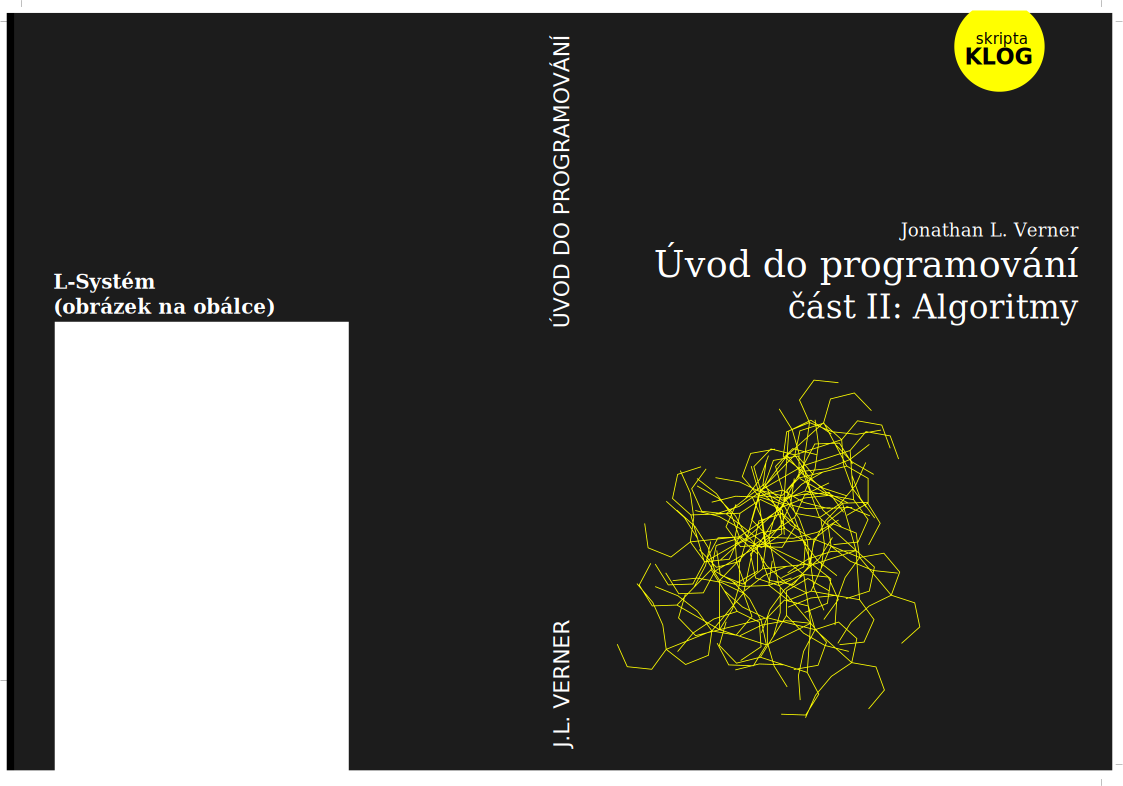
\includepdf[pages={1},noautoscale=true,fitpaper=true,offset=-8cm 0]{obalka-black.pdf}


\title{}

% \author{Jonathan Verner}
% \address{Department of Logic, Charles University\\
% Palachovo nám. 2\\ 116 38 Praha 1, Czech Republic}
% \email{jonathan.verner{@}ff.cuni.cz}
%\thanks{The author was partially supported by }

%\subjclass[2010]{Primary }
%\keywords{}

%\begin{abstract}
%\end{abstract}
%\maketitle
% \pagestyle{empty}

\headheight=12.4pt
\pagestyle{fancy}

%\hsize=16cm
\parindent=0cm
\parskip=0.2cm
\thispagestyle{empty}
\
\vskip1cm
Jonathan L. Verner, PhD.\\
Katedra Logiky\\
Filozofická fakulta UK\\
Palachovo náměstí 2\\
116 18 Praha 1
\vfill
\copyright\ Jonathan L. Verner, 2015 \\[3mm]
{\small Tato učebnice slouží jako skripta k letnímu semestru přednášky
\emph{Úvod do programování}, vypsané pod kódem ALG110006 na Katedře logiky FF UK
v letech 2011--2015. Jejich příprava byla podpořena projektem
OPVK CZ.1.07/2.2.00/28.0216 \emph{Logika: systémový rámec rozvoje oboru v ČR a
koncepce logických propedeutik pro mezioborová studia}\\}


\includegraphics[width=12cm]{logolink}
\eject
\thispagestyle{empty}
\
\vskip3cm
\begin{center}
 \sf\Huge Úvod do programování\\[1cm]
 \sf\Large část II: Algoritmy
\end{center}
\vfill
\eject

\lhead[\sf{\bf\thepage}]{\sf\nouppercase{\leftmark}}
\rhead[\sf\nouppercase{\leftmark}]{\sf\bf\thepage}
\cfoot{}

\tableofcontents

\setcounter{section}{3}
\fi
\section{Analýza jazyka}
V této kapitole se podíváme na problém analýzy jazyka.  Nepůjde nám o přirozené jazyky ---
to by přesahovalo možnosti úvodního kurzu --- ale o jazyky tzv. formální. Formální jazyky
jsou jazyky, které mají přesně specifikovánu syntax, t.j. co je a co není v jazyce přípustné. 
Co to znamená \emph{přesně} specifikovat? Dohodněme se, že pro naše účely to znamená,
že je možné o daném řetězci automaticky rozhodnout, zda je v jazyce přípustný či nikoliv.

\begin{doplneni}
Přirozené jazyky tuto podmínku nesplňují, protože přípustnost je nejednoznačná ---
na přípustnosti nějaké věty se často neshodnou ani lingvisté. Jednoduchým diagonálním 
argumentem však lze ``zkonstruovat'' jazyky, kde je přípustnost daná jednoznačně, nicméně
neexistuje algoritmus, který by o přípustnosti rozhodl.  Takové jazyky nás však zajímat nebudou.
\end{doplneni}

Příkladem formálního jazyka je třeba samotný Python. Dalším příkladem může být třeba
jazyk nějaké matematické teorie.  Nebo html, jazyk ve kterém se píší webové stránky. Toto
všechno jsou relativně komplikované jazyky, kterým odpovídají i (relativně) komplikované
rozhodovací algoritmy.  My si ukážeme několik jednodušších jazyků a algoritmy, které rozhodují o 
přípustnosti pro tyto jazyky. Nejprve se však budeme zabývat jednodušším problémem ---
vyhledáváním v textu.  Optimální algoritmus pro vyhledávání nás totiž navede k definici
tzv. regulárních jazyků.

\subsection*{Vyhledávání v textu}

Následující úlohu zná každý, kdo v textovém editoru někdy použil funkci ``najdi'' (find).

\begin{uloha}\label{uloha:substring}
Nalezněte v daném textu (posloupnosti znaků) všechny výskyty nějakého slova 
(věty, posloupnosti znaků).
\end{uloha}

První řešení, které nás napadne, může vypadat třeba takto:

\srchere{dumbfind}{Naivní Vyhledávání}

Vnější cyklus postupně prochází celý text a vnitřní cyklus na každé pozici testuje, zda
se tam nevyskytuje hledaná posloupnost. Tento vnitřní test provede nejvýše \(m\) operací,
kde \(m\) je délka hledaného řetězce. Celková složitost algoritmu je tedy \(O(n\cdot m)\), 
kde \(n\) je délka textu. Na první pohled nás napadne, že lépe to snad ani nejde. 
Uvědomme si však, že algoritmus dělá spoustu zbytečné práce. Představme si, že hledáme
řetězec {\tt aaaaa} ({\tt s}) v řetězci {\tt aaaazzzz} ({\tt text}). V první iteraci zjistíme, že na pozici {\tt 0}
se řetězec nenachází, protože páté písmeno je {\tt z} a ne {\tt a}. V tu chvíli však už je
zbytečné testovat všechny pozice do pátého písmena, protože náš řetězec žádné
{\tt z} neobsahuje.  Ve skutečnosti,  když testujeme výskyt řetězce na pozici {\tt tpos}
pro {\tt tpos >= 5}, všechny znaky {\tt text[tpos],...,text[tpos+4]} jsme už viděli, takže
znalost znaku {\tt text[tpos+5]} by nám teoreticky měla stačit k rozhodnutí, zda se
{\tt s} na pozici {\tt tpos} vyskytuje. Jak tuto informaci využít? Představme si, že každá
posloupnost {\tt p} čtyř znaků má přiřazeno nějaké číslo \(n_{\tt p}\). Pak lze sestrojit
tabulku, která nám pro každý znak {\tt z}, a číslo \(n_{\tt p}\) určí, 

\begin{itemize}
 \item zda je posloupnost {\tt p+z} (posloupnost {\tt p} následovaná znakem {\tt z}) je rovná hledané posloupnosti
 \item číslo \(n_{p[1:]+z}\) posloupnosti {\tt p+z} bez prvního znaku
\end{itemize}

Pokud bychom takovou tabulku měli, bylo by vyhledávání velmi jednoduché. Algoritmus
by vypadal třeba jako na výpisu \ref{alg:smartfind} (uvažujeme jednoduchý příklad, kdy
hledáme řetězec {\tt aab} v posloupnosti která sestává pouze ze znaků {\tt a} a {\tt b}).

\src[firstline=2]{smartfind}{Vyhledávání za pomoci tabulky}

Je lehké nahlédnout, že složitost je nyní lineární v délce textu, t.j. \(O(n)\). Problém je
však se sestrojením tabulky (a s její velikostí). Máme-li abecedu o \(k\) znacích
(v příkladu \ref{alg:smartfind} je \(k=2\)), a hledáme řetězec délky \(m\), pak naše tabulka
bude mít velikost \(k\cdot k^{m-1}\) a tedy její výroba bude trvat \(O(k^{m})\). 
Tím bychom vyměnili složitost \(O(n\cdot m)\) za \(O(n+k^{m})\), což není příliš výhodné.

\paragraph{Konečné automaty}

Naše tabulka je ale příliš veliká. Všimněte si například, že hodnoty odpovídající
\(n_{\tt p} = 1,2\) jsou stejné.  To napovídá, že by bylo možné ušetřit. Ukážeme, 
že tabulku lze nahradit komplikovanější strukturou, tzv. konečným automatem. 
Jeho výhoda spočívá v tom, že vhodný automat  lze vytvořit v čase \(O(m)\) 
(místo \(O(2^{m})\)). Co to je konečný automat?  Ukážeme si to nejprve na příkladě
jednoduchého konečného automatu --- zakódovaného zámku na kole. 

\begin{center}
 \includegraphics[width=5cm]{combination-lock}
\end{center}

Koncepčně má zámek dva stavy --- odemčeno a zamčeno.  Zadáním správného kódu 
ho člověk může ze stavu zamčeno přesunout
do stavu odemčeno.  Ve skutečnosti si však můžeme představit, že zámek má mimo
dvou základních stavů různé vnitřní stavy odpovídající různým možným kódovým
kombinacím. Jeden z těchto vnitřních stavů --- stav odpovídající správnému kódu ---
pak odpovídá globálnímu stavu odemčeno, ostatní odpovídají stavu zamčeno. 
Nastavením číslice na jednom z možných míst pak přesouváme zámek z jednoho
vnitřního stavu do jiného.

Obecná definice konečného automatu je zobecněním této konkrétní situace.

\begin{definition} \emph{Konečný automat} je dán množinou (vnitřních) stavů \(S\),
množinou vstupů (abecedou) \(\Sigma\), přechodovou funkcí \(f:S\times\Sigma\to S\),
množinou koncových stavů \(E\subseteq S\) a jedním počátečním stavem \(s^b\in S\).
\end{definition}

V případě zámku by množina vnitřních stavů byla množina všech 5 ciferných čísel,
Množina vstupů by byla množina všech dvojic (pozice, číslice), kde pozice je jedno z 
písmen A, B, C, D, E. Přechodová funkce pak odpovídá změně stavu při zadání jedné
číslice kódu. Koncový stav je jediný --- ten který odpovídá správnému kódu. 
Počáteční stav je náhodný zamčený stav, který byl nastaven při zamykání. 

Definujme ještě co to znamená výpočet. Intuitivně je to posloupnost stavů a vstupů
začínající v počátečním stavu a končící v nějakém koncovém stavu taková, že přechod 
mezi sousedními členy této posloupnosti je dán přechodovou funkcí:

\begin{definition} \label{def:vypocet}
Posloupnost stavů \(\overline{s}=\langle s_0,\ldots, s_n\rangle\)
a vstupů \(\overline{v}=\langle v_0,\ldots, v_{n-1}\rangle\) je výpočtem automatu 
\(A=(S_A,\Sigma_A,f_A, E_A,s_A^b)\) pokud \(s_0=s_A^b\), \(s_n\in E_A\) a pro \(1\leq i\leq n-1\) 
platí \(s_{i+1} = f(s_i,v_i)\).
\end{definition}

Když se zamyslíte nad algoritmem \ref{alg:smartfind} možná Vás napadne, že by se dal
popsat jako provádění výpočtu nějakého konečného automatu. Tabulka v tomto případě
prostě zadává přechodovou funkci.  Abychom dostali konečný automat, musíme ještě
doplnit počáteční stav, dva stavy odpovídající přečtení prvního znaku a koncový stav.
Výsledkem pak bude automat znázorněný na následujícím obrázku. Každé kolečko odpovídá
stavu, šipky mezi kolečky odpovídají přechodům mezi stavy daným vstupním písmenem.

\begin{center}
\begin{tikzpicture}[scale=0.2]
\tikzstyle{every node}+=[inner sep=0pt]
\draw [black] (11.3,-23.1) circle (3);
\draw (11.3,-23.1) node {$0$};
\draw [black] (34.3,-18.3) circle (3);
\draw (34.3,-18.3) node {$1$};
\draw [black] (43.3,-28.3) circle (3);
\draw (43.3,-28.3) node {$2$};
\draw [black] (26.9,-40.7) circle (3);
\draw (26.9,-40.7) node {$3$};
\draw [black] (21.7,-23.1) circle (3);
\draw (21.7,-23.1) node {$found$};
\draw [black] (21.7,-23.1) circle (2.4);
\draw [black] (36.3,-5.3) circle (3);
\draw (36.3,-5.3) node {$start$};
\draw [black] (24.5,-12.2) circle (3);
\draw (24.5,-12.2) node {$a$};
\draw [black] (42.7,-13.2) circle (3);
\draw (42.7,-13.2) node {$b$};
\draw [black] (33.71,-6.81) -- (27.09,-10.69);
\fill [black] (27.09,-10.69) -- (28.03,-10.71) -- (27.53,-9.85);
\draw (29.35,-8.25) node [above] {$a$};
\draw [black] (38.19,-7.63) -- (40.81,-10.87);
\fill [black] (40.81,-10.87) -- (40.7,-9.93) -- (39.92,-10.56);
\draw (38.94,-10.68) node [left] {$b$};
\draw [black] (22.19,-14.11) -- (13.61,-21.19);
\fill [black] (13.61,-21.19) -- (14.55,-21.07) -- (13.91,-20.29);
\draw (16.84,-17.16) node [above] {$a$};
\draw [black] (14.3,-23.1) -- (18.7,-23.1);
\fill [black] (18.7,-23.1) -- (17.9,-22.6) -- (17.9,-23.6);
\draw (16.5,-23.6) node [below] {$b$};
\draw [black] (8.816,-21.438) arc (263.94407:-24.05593:2.25);
\draw (6.88,-16.75) node [above] {$a$};
\fill [black] (11.11,-20.12) -- (11.69,-19.38) -- (10.7,-19.27);
\draw [black] (45.15,-14.924) arc (49.44438:-109.20303:15.858);
\fill [black] (29.62,-41.95) -- (30.21,-42.68) -- (30.54,-41.74);
\draw (49.24,-36.1) node [right] {$a$};
\draw [black] (42.82,-16.2) -- (43.18,-25.3);
\fill [black] (43.18,-25.3) -- (43.65,-24.48) -- (42.65,-24.52);
\draw (43.56,-20.74) node [right] {$b$};
\draw [black] (22.55,-25.98) -- (26.05,-37.82);
\fill [black] (26.05,-37.82) -- (26.3,-36.91) -- (25.34,-37.2);
\draw (23.53,-32.49) node [left] {$a$};
\draw [black] (24.62,-23.8) -- (40.38,-27.6);
\fill [black] (40.38,-27.6) -- (39.72,-26.92) -- (39.49,-27.9);
\draw (31.74,-26.28) node [below] {$b$};
\draw [black] (27.05,-13.79) -- (31.75,-16.71);
\fill [black] (31.75,-16.71) -- (31.34,-15.87) -- (30.81,-16.72);
\draw (28.3,-15.75) node [below] {$b$};
\draw [black] (36.31,-20.53) -- (41.29,-26.07);
\fill [black] (41.29,-26.07) -- (41.13,-25.14) -- (40.39,-25.81);
\draw (39.34,-21.84) node [right] {$b$};
\draw [black] (27.142,-37.71) arc (173.41001:150.02731:43.825);
\fill [black] (27.14,-37.71) -- (27.73,-36.97) -- (26.74,-36.86);
\draw (28.3,-28.3) node [left] {$a$};
\draw [black] (24.91,-38.45) -- (13.29,-25.35);
\fill [black] (13.29,-25.35) -- (13.45,-26.28) -- (14.19,-25.61);
\draw (19.64,-30.45) node [right] {$a$};
\draw [black] (34.144,-21.295) arc (-5.17826:-31.38442:39.268);
\fill [black] (34.14,-21.3) -- (33.57,-22.05) -- (34.57,-22.14);
\draw (33.09,-30.76) node [right] {$b$};
\draw [black] (40.91,-30.11) -- (29.29,-38.89);
\fill [black] (29.29,-38.89) -- (30.23,-38.81) -- (29.63,-38.01);
\draw (34.05,-34) node [above] {$a$};
\draw [black] (45.015,-30.747) arc (62.74616:-225.25384:2.25);
\draw (44.75,-35.58) node [below] {$b$};
\fill [black] (42.4,-31.15) -- (41.59,-31.63) -- (42.48,-32.09);
\end{tikzpicture}
\end{center}

Jak jsme poznamenali již dříve a je z obrázku vidět, že stavy \(1\) a \(2\) jsou v podstatě ekvivalentní a mohli bychom je sloučit
dohromady.  Ve skutečnosti lze ale celý automat ještě podstatně zjednodušit tak, aby
měl přesně o jeden stav více než je délka hledaného řetězce (\(m\)).  Stavy automatu
na obrázku odpovídají všem možným nejvýše dvouprvkovým posloupnostem písmen 
{\tt a,b}.  Například stav \(0\) odpovídá posloupnosti {\tt aa} zatímco třeba stav \(3\)
odpovídá posloupnosti {\tt ba}. Základní myšlenka spočívá v tom, že zahodíme všechny
stavy, které neodpovídají žádnému počátečnímu úseku hledaného řetězce.
Získáme tak automat znázorněný následujícím obrázkem:

\begin{center}
\begin{tikzpicture}[scale=0.2]
\tikzstyle{every node}+=[inner sep=0pt]
\draw [black] (42.6,-21.1) circle (3);
\draw (42.6,-21.1) node {$0$};
\draw [black] (57.7,-21.1) circle (3);
\draw (57.7,-21.1) node {$found$};
\draw [black] (57.7,-21.1) circle (2.4);
\draw [black] (10.8,-21.1) circle (3);
\draw (10.8,-21.1) node {$\emptyset$};
\draw [black] (25.2,-21.1) circle (3);
\draw (25.2,-21.1) node {$a$};
\draw [black] (28.2,-21.1) -- (39.6,-21.1);
\fill [black] (39.6,-21.1) -- (38.8,-20.6) -- (38.8,-21.6);
\draw (33.9,-21.6) node [below] {$a$};
\draw [black] (45.6,-21.1) -- (54.7,-21.1);
\fill [black] (54.7,-21.1) -- (53.9,-20.6) -- (53.9,-21.6);
\draw (50.15,-21.6) node [below] {$b$};
\draw [black] (40.116,-19.438) arc (263.94407:-24.05593:2.25);
\draw (38.18,-14.75) node [above] {$a$};
\fill [black] (42.41,-18.12) -- (42.99,-17.38) -- (42,-17.27);
\draw [black] (12.482,-18.638) arc (134.70674:45.29326:7.844);
\fill [black] (12.48,-18.64) -- (13.4,-18.43) -- (12.7,-17.72);
\draw (18,-15.87) node [above] {$b$};
\draw [black] (13.8,-21.1) -- (22.2,-21.1);
\fill [black] (22.2,-21.1) -- (21.4,-20.6) -- (21.4,-21.6);
\draw (18,-21.6) node [below] {$a$};
\draw [black] (55.443,-23.075) arc (-51.3352:-128.6648:33.922);
\fill [black] (13.06,-23.08) -- (13.37,-23.97) -- (13.99,-23.18);
\draw (34.25,-31.01) node [below] {$b,a$};
\end{tikzpicture}
\end{center}

Zbývá ještě ukázat, že takový automat umíme sestrojit v čase \(O(m)\).  Sestrojit stavy
a základní ``dopředné'' šipky spojující tyto stavy od nejkratšího k nejdelšímu je jednoduché.
Potřebujeme však ještě dodat šipky jdoucí ``zpět''.  Řekněme, že jsme  v nějakém stavu \(s\) 
který odpovídá řetězci {\tt r}. Abychom mohli správně dodat šipky jdoucí ``zpět'', potřebovali
bychom znát stav \(s^\prime\) odpovídající řetězci {\tt r[1:]} (každá šipka jdoucí zpět totiž bude 
odpovídat nějaké šipce ze stavu \(s^\prime\)). Není však problém si tento stav uložit v nějaké
pomocné proměnné a tuto proměnnou postupně aktualizovat.  Celý algoritmus v Pythonu
(včetně funkce find) lze nalézt na výpisu \ref{alg:optimalfind}.

\src[firstline=3]{optimalfind}{Vyhledávání pomocí konečných automatů}

Pro zájemce dodejme, že existuje ještě jiný algoritmus, tzv. Boyer-Moore algoritmus, 
který řeší úlohu \ref{uloha:substring} také v čase \(O(m+n)\) ale v praxi je rychlejší než 
algoritmus \ref{alg:optimalfind}.

\subsection*{Regulární jazyky}

V předchozím odstavci jsme zavedli pojem konečného automatu a ukázali, jak lze konečné
automaty využít pro rychlé hledání v textu. Nicméně samotný pojem konečného automatu 
je zajímavý i teoreticky, protože se dá ukázat, že charakterizuje třídu regulárních jazyků. 

\begin{definition} Je-li \(\Sigma\) množina znaků (\emph{abeceda}), značíme \(\Sigma^*\) množinu všech
(konečných) posloupností prvků množiny \(\Sigma\). Prvkům množiny \(\Sigma^*\) budeme říkat
\emph{slova}.  \emph{Jazykem} v abecedě \(\Sigma\) pak rozumíme libovolnou podmnožinu \(L\subseteq\Sigma^*\).
\end{definition}

\begin{definition}  Třída \emph{regulárních jazyků} nad abecedou \(\Sigma\) je nejmenší třída \(\mathcal L\) splňující:
\begin{itemize}
  \item[(i)] Prázdný jazyk je prvkem \(\mathcal L\),
 \item[(ii)] Pro každý znak \(a\in\Sigma\) je \(\{a\}\in\mathcal L\),
 \item[(iii)] Třída \(\mathcal L\) je uzavřená na sjednocení a konkatenaci (jsou-li \(A,B\in\mathcal L\), pak jejich konatenace,
                     značená \(A\cdot B\), je jazyk sestávající ze slov tvaru \(w_Aw_B\), kde \(w_A\in A\) a \(w_B\in B\)).
 \item[(iv)] Třída \(\mathcal L\) je uzavřená na Kleeneho hvězdičku (je-li \(A\in\mathcal L\), pak i jazyk \(A^*\) je prvkem
                     \(\mathcal L\), kde \(A^*\) je nejmenší nadmnožina \(A\) obsahující prázdnou množinu a uzavřená na konkatenaci).
\end{itemize}
\end{definition}

Tato definice vypadá velmi abstraktně. Nicméně je překvapivé, že má mnoho různých ekvivalentních reformulací.
Jedna možná definice využívá konečné automaty:

\begin{theorem} Jazyk \(L\) je \emph{regulární}, pokud existuje konečný automat \(A\) takový, že
\(L\) je množinou slov \(w\) takových, že existuje posloupnost stavů \(\overline{s}\), že \((\overline{s},w)\) je
výpočtem (viz \ref{def:vypocet}) automatu \(A\). 
\end{theorem}

Nabízí se otázka, zda je každý jazyk regulární. Jednoduchým argumentem se můžeme přesvědčit, že nikoliv: všech jazyků
je totiž nespočetně (kontinuum), ale konečných automatů je jen spočetně (každý konečný automat je konečný objekt).
Není příliš těžké dokonce přímo sestrojit neregulární jazyk.

\begin{cviceni}\label{cv:zavorky}
Ukažte, že jazyk nad abecedou \(\Sigma=\{(,)\}\) sestávající ze správně uzávorkovaných výrazů, nemůže
být regulární.  (Hint: uvažte řetězec začínající \(n+1\)-otevřenými závorkami, kde \(n\) je počet stavů daného automatu.)
\end{cviceni}

\paragraph{Regulární výrazy}
Ukážeme si ještě jinou ekvivalentní definici regulárního jazyka, která je bližší původní definici a používá pojem regulárního výrazu. 
Tento pojem zavedl americký matematik \person{Kleene} a umožňuje velmi kompaktní popis regulárních jazyků. Každému regulárnímu
výrazu \(R\) odpovídá jazyk \(L(R)\) dle následující definice

\begin{definition} \emph{Regulární výraz} nad abecedou \(\Sigma\) 
(neobsahující znaky \(\varepsilon,(,),|,*\)) je definován rekurzivně:
\begin{itemize}
 \item \(\emptyset, \varepsilon\) jsou regulární výrazy, \(L(\emptyset)=\emptyset, L(\varepsilon) = \{\emptyset\}\),  t.j. prázdný jazyk a jazyk sestávající z prázdného slova,
 \item každý znak \(a\in\Sigma\) je regulárním výrazem, \(L(a) = \{a\}\),
 \item je-li \(r\) regulární výraz, pak i \((r)\) je regulární výraz a \(L((r)) = L(r)\),
 \item jsou-li \(r,s\) dva regulární výrazy, pak \(r|s\) a \(rs\) je regulární výraz a \(L(r|s)=L(r)\cup L(s)\),\(L(rs)=L(r)\cdot L(s)\) (alternace a konkatenace)
 \item je-li \(r\) regulární výraz, pak \(r^*\) je regulární výraz a \(L(r^*) = L(r)^*\) (Kleeneho hvězdička).
\end{itemize}
\end{definition}

Aby se předešlo zbytečnému množství závorek je stanovena standardní priorita operací: Kleeneho  hvězdička má nejvyšší prioritu, pak konkatenace a
nakonec alternace. 

\begin{example} Je-li \(\Sigma=\{a,b,c\}\), pak \(r=ac^*(aa|bb)^*\) je regulární výraz popisující jazyk sestávající ze slov začínajících písmenem \(a\), pokračujících libovolným počtem znaků \(c\)
a pak libovolným počtem dvojic znaků \(aa\) nebo \(bb\).
\end{example}

Následující věta říká, že regulární výrazy přesně popisují regulární jazyky.

\begin{theorem} Jazyk \(L\) nad abecedou \(\Sigma\) je regulární právě když existuje regulární výraz \(r\) takový, že \(L=L(r)\).
\end{theorem}


\subsection*{Aritmetické výrazy}
Ve cvičení \ref{cv:zavorky} jsme uvedli, že jazyk sestávající ze slov obsahujících
stejně otevřených jako zavřených závorek není regulární. To naznačuje, že 
mnoho zajímavých jazyků pravděpodobně regulárních nebude. Typickým reprezentantem
je například jazyk sestávající z aritmetických výrazů, kterým se nyní budeme
podrobněji zabývat. Že je to neregulární jazyk je vidět z toho, že nejen že
musí obsahovat stejný počet otevřených jako zavřených závorek, tyto závorky
navíc musí být správně poskládané. S aritmetickými výrazy se každý z vás nejspíš
setkal již někdy v první třídě základní školy a máte intuitivní představu o tom, 
co to aritmetický výraz je. Abychom s nimi mohli pracovat bude užitečné tuto
intuitivní představu zpřesnit do formální definice. Pro jednoduchost budeme
uvažovat pouze aritmetické výrazy, ve kterých se nevyskytují proměnné a jediné
povolené operace jsou sčítání, odčítání, násobení a dělení. Formálně tedy budou 
aritmetické výrazy řetězce nad abecedou 
\(\Sigma = \{0,1,2,3,4,5,6,7,8,9,+,-,*,/,(,)\}\). Nejjednodušším
aritmetickým výrazem je nějaké libovolné číslo (řetězec číslic, t.j. 
neprázdný prvek jazyka \(\{0,1,2,3,4,5,6,7,8,9\}^*\)).
Tyto výrazy (t.j. čísla) budeme nazývat \emph{atomickými výrazy}. 

\begin{definition} Jazyk aritmetických výrazů je nejmenší
podmnožina \(\Sigma^*\) která obsahuje všechny atomické výrazy a je
uzavřena na následující operaci:
\begin{itemize}
 \item Jsou-li \(a,b\) dva řetězce a \(o\in\{+,-,*,/\}\) pak první
       operace (OP1) je definovaná takto:
       \[
          OP1(a,b,o)=aob
       \]
       
       t.j. výsledkem je řetězec sestávající
       z konkatenace levé závorky, řetězce a, symbolu op, řetězce b a 
       pravé závorky.
  \item Je-li \(a\) řetězec, pak druhá operace (OP2) je definovaná
       takto:
       \[
          OP2(a) = (a)
       \]
       t.j. výsledek je konkatenací levé závorky, řetězce \emph{a} a pravé
       závorky.
\end{itemize}
\end{definition}

\paragraph{Stromová reprezentace}

Každý aritmetický výraz tedy vznikne z atomických výrazů (čísel) postupným
aplikováním operace OP1 (aritmetické operace) resp. OP2 (uzávorkování). 
Tuto postupnou výstavbu aritmetického výrazu si můžeme představit jako 
(v našem případě binární) strom. V koředni stromu je výsledný výraz a poslední 
provedená operace, kterou byl získán. Jeho dětmi jsou pak ty jednodušší výrazy, 
ze kterých byl pomocí této operace vytvořen. V listech stromu jsou pak atomické
výrazy. Nejlépe to je vidět na nějakém příkladě. Například stavba výrazu 
\((8+7)*5\) je znázorněna následujícím stromem:

\begin{center}
\Tree [.'((8+7)*5)',OP1* [.'(8+7)',OP2 [.'8+7',OP1+ [.'8' ]  [.'7' ] ] ] [.'5' ] ]
\end{center}

Tento strom můžeme ještě trochu zjednoduššit tím, že si v uzlech budeme
pamatovat pouze operace a zahodíme všechny neatomické výrazy:

\begin{center}
\Tree [.* [.() [.+ [.8 ] [.7 ] ] ] [.5 ] ]
\end{center}

Dalšího zjednoduššení můžeme dosáhnout, pokud nám nezáleží na rozlišení výrazů, 
které se liší pouze různým ekvivalentním uzávorkováním. V takovém případě můžeme
prostě zahodit uzly s druhou operací. Získáme tak strom:

\begin{center}
\Tree [.* [.+ [.8 ] [.7 ] ] [.5 ] ]
\end{center}

Je však dobré si uvědomit, že v tomto případě již došlo ke ztrátě informace:
stejný strom by nám totiž vyšel i pro výraz '(8+7)*(5)'. Pro většinu aplikací
je však důležitá hodnota výrazu, kterou tato ztráta neovlivní. Uvědomte si,
že výraz 8+(7*5), který má jinou hodnotu, dá ve skutečnosti jiný strom, ačkoliv 
se od původního výrazu liší pouze uzávorkováním; toto uzávorkování je totiž
\emph{neekvivalentní}. 

Se závorkami souvisí ještě jeden problém. Výše zmíněná výstavba výrazu není
vždy jednoznačná. Například výrazu \(8+7*5\) odpovídají následující dva
stromy:

\begin{center}
\Tree [.* [.+ [.8 ] [.7 ] ] [.5 ] ] 
\hskip2cm
\Tree [.+ [.8 ] [.* [.7 ] [.5 ] ] ]
\end{center}

K tomuto problému se dostaneme za chvíli, až se budeme zabývat konstrukcí
těchto stromů. 

\paragraph{Vyhodnocování výrazů} Předpokládejme však na chvíli, že strom pro 
daný aritmetický výraz již máme v Pythonu k dispozici, například pro výraz 
'(8+7)*5' máme tedy strom

\begin{python}
 >>> T = ['*',['+',[8,None,None],[7,None,None]],[5,None,None]]
\end{python}

V tuto chvíli je relativně jednoduché výraz vyhodnotit. Vyhodnocování bude
probíhat rekurzivně tak, že spočteme hodnotu každého uzlu, který odpovídá nějakému
podvýrazu. Hodnota listů, t.j. atomických výrazů, je prostě dané
číslo. Hodnota vnitřních uzlů se pak spočte aplikací operace uložené v uzlu na
hodnoty jeho dětí. V pythonu to může vypadat takto:

\begin{python}
def eval_tree(T):
    D,L,R = T
    
    # Hodnota listu je v něm uložená
    if L is None and R is None:
        return D
        
    # Rekurzivně spočtěme hodnotu dětí
    LVal = eval_tree(L)
    RVal = eval_tree(R)
    
    # Aplikujme operaci D
    if D == '+':
        return LVal + RVal
    if D == '-':
        return LVal - RVal
    if D == '*':
        return LVal * RVal
    if D == '/':
        return LVal / RVal    
\end{python}

Stromová reprezentace se hodí pro další zpracování, pro uživatele ale není 
příliš čitelná. Proto je užitečné mít funkci, která strom převede zpět na
aritmetický výraz. I tuto funkce napíšeme snadno za pomoci rekurze:

\begin{python}
def tree_to_expr_naive(T):
    D,L,R = T
    
    if L is None and R is None:
        return str(D)
    
    return tree_to_expr_naive(L) + D + tree_to_expr_naive(R)
\end{python}

Zde však narazíme na výše zmíněný problém související s tím, že jsme zahodili 
závorky. Náš strom totiž dá výraz výraz '8+7*5', který je možno číst dvěmi
způsoby jako '8+(7*5)' či '(8+7)*5'. Konvence o prioritách operací pak preferuje
druhou variantu, která však odpovídá jinému stromu! Abychom se této dvojznačnosti
vyhli, budeme muset na vhodných místech vypsat závorky. Správnější tedy
bude napsat funkci takto:

\begin{python}
def tree_to_expr_inorder(T):
    D,L,R = T
    
    if L is None and R is None:
        return str(D)
    
    ret = '('
    ret = ret + ' ' + tree_to_expr_inorder(L)
    ret = ret + ' ' + D
    ret = ret + ' ' + tree_to_expr_inorder(R)
    ret = ret + ' )'
    return ret
\end{python}

Tato funkce vrátí pro původní strom výraz '( ( 8 + 7 ) * 5 )'. Kdyby daný výraz psal
člověk, pravděpodobně by vynechal vnější závorky. Přebytečné závorky by samozřejmě
šlo odstranit, bylo by to ale příliš komplikované, proto se smíříme s tím, že
naše funkce občas závorkuje příliš horlivě. 

\paragraph{Prefixová a postfixová notace} Zastavme se ještě u funkce
{\tt tree\_to\_expr\_inorder}. Funkce postupně rekurzivně prochází uzly stromu.
Když přijde do daného uzlu, nejprve rekurzivně převede levý podstrom na výraz,
k tomuto výrazu přidá operaci D a pak rekurzivně převede pravý podstrom a připojí
ho nakonec. Co by se stalo, kdybychom prohodili řádky 8 a 9?  T.j. při příchodu
do uzlu bychom nejprve ``vypsali'' operaci v daném uzlu a teprve pak se zabývali
podstromy. Výsledkem by byl následující výraz
\begin{center}
 ( * ( + 8 7 ) 5 )
\end{center}
Ačkoliv to na první pohled nemusí vypadat příliš užitečně, má tento zápis
svůj smysl a dokonce i jméno --- říká se mu prefixový zápis (a odpovídajícímu 
způsobu procházení stromu se říká preorder). V tomto zápise se nejprve zapíše
operace a po ní teprve následují operandy. Výhoda tohoto zápisu je (ačkoliv to možná
není hned vidět), že se obejde bez závorek a tudíž odpadají nejednoznačnosti, 
které se závorkami souvisí. Navíc je relativně jednoduché tento zápis převést
zpět na odpovídající strom. 


\paragraph{Bezkontextové gramatiky}

\ifx\ucebnice\undefined
\renewcommand{\refname}{\textbf{Literatura}}
\bibliographystyle{mujstyl}
\bibliography{ref}
\renewcommand{\glossarypreamble}{Biografické údaje jsou převzaté z \href{http://www.wikipedia.org}{Wikipedie}.}
\printglossary[type=person,title={Lidé}]
\end{document}
\fi
